%!TEX TS-program = pdflatex
%!TEX TS-options = -shell-escape
%!TEX root = qrcode.tex
%!TEX TS-options = -shell-escape
%!BIB programm = biber
\documentclass[%
	paper=a4,
	fontsize=10,
	DIV=13,
	chapterprefix=true,
	headinclude,
	footinclude,
	headheight=.6cm,
	headings=optiontohead,
	toc=bibliography,toc=listof,
	ngerman,
	draft=true,
]{scrbook}
\usepackage{scrtime}
\usepackage{etex}
\usepackage{shellesc}
\usepackage[final]{graphicx}

%-- typografische Verbesserungen, Codierungskram, Schriftwahl und erste Mathepakete
%----------------------------------------------------------------------------------------
\usepackage[utf8]{inputenc}

%-- verschiedene Schriftarten zur Auswahl
% \usepackage[lining,semibold]{libertine}
% \usepackage[proportional,scaled=1.0]{erewhon}
% \usepackage{concmath}
% \usepackage[default]{droidserif}
\usepackage[oldstyle]{XCharter}
% \usepackage[rm]{merriweather}
% \usepackage[default,regular,bold,osf]{sourceserifpro}

%-- Sans- und Mono-Schriftart
% \usepackage[rm,light]{roboto}
\usepackage[scale=0.90]{sourcecodepro}
\usepackage[scale=1.00]{sourcesanspro}
% \usepackage[sb,lining,scale=.92]{FiraSans}
% \usepackage[lining,scale=.87]{FiraMono}

\usepackage[T1]{fontenc}
\usepackage{textcomp} % verhindert ein paar Fehler bei den Fonts
\usepackage[newcommands]{ragged2e} % besserer Flattersatz

\usepackage{mathtools} 
\usepackage[bigdelims]{newtxmath} % Mathe Schriftart
\DeclareMathSymbol{,}{\mathpunct}{operators}{"2C}   % Fix für fehlerhaftes Spacing von Kommas, siehe http://tex.stackexchange.com/a/160790/67086
\usepackage{fontawesome}
\usepackage{babel}
\usepackage[babel=true,final,tracking=smallcaps]{microtype} 
\SetTracking{ encoding = *, shape = sc}{ 45 } % aktiviert ein nicht übertriebenes Tracking von SmallCaps
\DisableLigatures{encoding = T1, family = tt* } % deaktiviere alle Ligaturen für Mono-Spacing-Fonts
\usepackage[german=quotes]{csquotes}
%----------------------------------------------------------------------------------------

%-- Seiteneinrichtung
%----------------------------------------------------------------------------------------
% \setlength\parindent{0pt}             % und ohne Einrueckung
% \setlength\parskip{1.5\medskipamount} % Absaetze abgesetzt
% Das obige in richtig:
% \usepackage{parskip}
%----------------------------------------------------------------------------------------

%-- Konfiguration von Farben
%----------------------------------------------------------------------------------------
\usepackage[usenames,x11names,final]{xcolor} % Die Optionen definieren zusätzliche Farben (siehe Dokumentation)
\definecolor{light_gray}{gray}{0.6}
\definecolor{blackberry}{rgb}{0.53, 0.0, 0.25}
\definecolor{FB_blue}{RGB}{60,89,153}
%----------------------------------------------------------------------------------------

%-- Einrichtung von TikZ
%----------------------------------------------------------------------------------------
\usepackage{tikz}
\usetikzlibrary{shapes.geometric}
\usetikzlibrary{arrows.meta}
%----------------------------------------------------------------------------------------

%-- Kopf- und Fußzeilen und allgemeine KOMO-Skript Formatierung
%----------------------------------------------------------------------------------------
\addtokomafont{chapter}{\Huge}
\addtokomafont{chapterprefix}{\LARGE\rmfamily\scshape}
\addtokomafont{captionlabel}{\sffamily\bfseries}
\usepackage[%
	headsepline=1pt,
	automark,
	draft=false,
	]%
{scrlayer-scrpage}
\pagestyle{scrheadings}
% \clearscrheadfoot % Standardkonfiguration löschen
% \setkomafont{pageheadfoot}{\sffamily}
% \renewcommand*\chaptermarkformat{\thechapter\autodot\enskip}
\ohead{
\includegraphics[height=0.6 cm,keepaspectratio]{images/wwulogo.pdf}}
\ihead{\rule{0cm}{0.6cm}\headmark}
\ofoot*{\Large\sffamily\thepage}
\ifoot{\color{light_gray}Praktikum Computer Vision}
%----------------------------------------------------------------------------------------

%-- Satzspiegel neu berechnen
%----------------------------------------------------------------------------------------
\KOMAoptions{DIV=last}
%----------------------------------------------------------------------------------------

%-- Konfiguration von Biblatex
%----------------------------------------------------------------------------------------
\usepackage[%
	backend=biber,
	sortlocale=auto,
	natbib,
	hyperref,
	backref,
	style=alphabetic,
	]%
{biblatex}
\renewcommand*{\mkbibnamefamily}[1]{%
  \ifmknamesc{\textsc{#1}}{#1}}

\renewcommand*{\mkbibnameprefix}[1]{%
  \ifboolexpr{ test {\ifmknamesc} and test {\ifuseprefix} }
    {\textsc{#1}}
    {#1}}

\def\ifmknamesc{%
  \ifboolexpr{ test {\ifcurrentname{labelname}}
               or test {\ifcurrentname{author}}
               or ( test {\ifnameundef{author}} and test {\ifcurrentname{editor}} ) }}
\addbibresource{quellen.bib}
%----------------------------------------------------------------------------------------

%-- Konfiguration von Hyperref 
%----------------------------------------------------------------------------------------
\usepackage[%
	hidelinks,
	pdfpagelabels,
	bookmarksopen=true,
	bookmarksnumbered=true,
	linkcolor=black,
	urlcolor=SkyBlue2,
	plainpages=false,
	pagebackref,
	citecolor=black,
	hypertexnames=true,
	pdfborderstyle={/S/U},
	linkbordercolor=SkyBlue2,
	colorlinks=false,
	final,
	backref=false,
	pdfencoding=auto]{hyperref}
\hypersetup{final}
%----------------------------------------------------------------------------------------
	
	
%-- Schöne Emailadressen setzen (nach http://tex.stackexchange.com/a/663/67086)
%----------------------------------------------------------------------------------------
\catcode`\_=11\relax
\newcommand\email[1]{\_email #1\q_nil}
\def\_email#1@#2\q_nil{%
  \href{mailto:#1@#2}{{\emailfont #1\emailampersat #2}}
}
\newcommand\emailfont{\ttfamily}
\newcommand\emailampersat{{\fontsize{10.9pt}{12pt}\selectfont\sffamily@}}
\catcode`\_=8\relax
%----------------------------------------------------------------------------------------

%-- Für Testzwecke, Marginnotes und Todos
%----------------------------------------------------------------------------------------
\usepackage{blindtext}
\usepackage[fulladjust]{marginnote}
\renewcommand*{\marginfont}{\itshape\footnotesize}
\usepackage[textsize=small,obeyDraft,color=Red1!80!OrangeRed1!80]{todonotes}
\renewcommand*{\raggedleftmarginnote}{\RaggedLeft}
\renewcommand*{\raggedrightmarginnote}{\RaggedRight}
\deffootnote[1.5em]{1.5em}{1.5em}{\textsuperscript{\thefootnotemark}\ } % extra Leerzeichen in Fußnote
%----------------------------------------------------------------------------------------

%-- Für Auflistungen und Tabellen
%----------------------------------------------------------------------------------------
\usepackage{multicol}
\usepackage[shortlabels]{enumitem}
\setlist{itemsep=0pt}
\setlist[enumerate]{font=\bfseries}
\setlist[description]{font=\bfseries}
\usepackage{tabularx}
\usepackage{booktabs}
\usepackage{longtable}
%----------------------------------------------------------------------------------------

%-- Für Abbildungen
%----------------------------------------------------------------------------------------
\usepackage{subcaption}
%----------------------------------------------------------------------------------------

%-- Theorem, Definition, Proof...
%----------------------------------------------------------------------------------------
\newtheorem{theorem}{Definition}[section]
\newtheorem{corollary}{Korollar}[theorem]
\newtheorem{lemma}[theorem]{Lemma}


%-- Listings
%----------------------------------------------------------------------------------------
% -- Bei 'shellesc' Problemen ab hier auskommentieren
\usepackage{tcolorbox}
\tcbuselibrary{breakable}
\tcbuselibrary{listingsutf8}
\tcbuselibrary{skins}
\tcbuselibrary{xparse}
% -- bis hier, stattdessen die folgende Zeile einkommentieren:
% \usepackage{listingsutf8}
\lstset{language=java}

\lstdefinestyle{customJava}{
	belowcaptionskip=1\baselineskip,
	breaklines=true,
	language=java,
	showstringspaces=false,
	basicstyle=\footnotesize\ttfamily,
	keywordstyle=\bfseries\color{green!40!black},
	commentstyle=\itshape\color{purple!40!black},
	identifierstyle=\color{blue},
	stringstyle=\color{orange},
	numbers=right,
	numbersep=1pt,
	numberstyle=\tiny\ttfamily\color{gray},
	inputencoding=utf8/latin1,
	tabsize=4,
}
\lstdefinestyle{jooqJava}{
	belowcaptionskip=1\baselineskip,
	breaklines=true,
	language=java,
	showstringspaces=false,
	basicstyle=\footnotesize\ttfamily,
	keywordstyle=\bfseries\color{green!40!black},
	commentstyle=\itshape\color{purple!40!black},
	identifierstyle=\color{blue},
	stringstyle=\color{orange},
	numbers=right,
	numbersep=1pt,
	numberstyle=\tiny\ttfamily\color{gray},
	inputencoding=utf8/latin1,
	tabsize=4,
	morekeywords={join,on,eq,selectFrom,where,and,orderBy,asc,fetch},
}
\lstdefinestyle{SQL}{
	belowcaptionskip=1\baselineskip,
	breaklines=true,
	language=sql,
	showstringspaces=false,
	basicstyle=\footnotesize\ttfamily,
	keywordstyle=\bfseries\color{green!40!black},
	commentstyle=\itshape\color{purple!40!black},
	identifierstyle=\color{blue},
	stringstyle=\color{orange},
	numbers=right,
	numbersep=1pt,
	numberstyle=\tiny\ttfamily\color{gray},
	inputencoding=utf8/latin1,
	morekeywords={BIGINT,CONFLICT},
}

\lstdefinestyle{customXML}{
	belowcaptionskip=1\baselineskip,
	breaklines=true,
	language=XML,
	showstringspaces=false,
	basicstyle=\footnotesize\ttfamily,
	keywordstyle=\bfseries\color{green!40!black},
	commentstyle=\itshape\color{purple!40!black},
	identifierstyle=\color{blue},
	stringstyle=\color{orange},
	numbers=right,
	numbersep=1pt,
	numberstyle=\tiny\ttfamily\color{gray},
	inputencoding=utf8/latin1,
}

\lstdefinestyle{customHTML}{
	belowcaptionskip=1\baselineskip,
	breaklines=true,
	language=HTML,
	showstringspaces=false,
	basicstyle=\footnotesize\ttfamily,
	keywordstyle=\bfseries\color{green!40!black},
	commentstyle=\itshape\color{purple!40!black},
	identifierstyle=\color{blue},
	stringstyle=\color{orange},
	numbers=right,
	numbersep=1pt,
	numberstyle=\tiny\ttfamily\color{gray},
	inputencoding=utf8/latin1,
}

\lstdefinestyle{CPP}{
	belowcaptionskip=1\baselineskip,
	breaklines=true,
	language=C++,
	showstringspaces=false,
	basicstyle=\footnotesize\ttfamily,
	keywordstyle=\bfseries\color{green!40!black},
	commentstyle=\itshape\color{purple!40!black},
	identifierstyle=\color{blue},
	stringstyle=\color{orange},
	numbers=right,
	numbersep=1pt,
	numberstyle=\tiny\ttfamily\color{gray},
	inputencoding=utf8/latin1,
	tabsize=4,
}

% -- Bei 'shellesc' Problemen ab hier auskommentieren
\newtcbinputlisting[%
	auto counter,
	number within=chapter,
	list inside=lol,
	]{\inputCode}[3][]{%
	listing file={#2},
	breakable,
	enhanced,
	listing only,
	top=1mm,bottom=1mm,
	label type=listing,
	before skip=\baselineskip,
	after=\vspace{\baselineskip}\noindent,
	title=Listing~\thetcbcounter.:\ #3,#1
}
\DeclareDocumentCommand{\inputJava}{ O{} O{} O{} m }{%
	\inputCode[listing options={style=customJava,#2},#1]{#4}{#3}%
}
\DeclareDocumentCommand{\inputXML}{ O{} O{} O{} m }{%
	\inputCode[listing options={style=customXML,#2},#1]{#4}{#3}%
}
\DeclareDocumentCommand{\inputHTML}{ O{} O{} O{} m }{%
	\inputCode[listing options={style=customHTML,#2},#1]{#4}{#3}%
}
\DeclareDocumentCommand{\inputSQL}{ O{} O{} O{} m }{%
	\inputCode[listing options={style=SQL,#2},#1]{#4}{#3}%
}
\DeclareDocumentCommand{\inputJooqJava}{ O{} O{} O{} m }{%
	\inputCode[listing options={style=jooqJava,#2},#1]{#4}{#3}%
}

\DeclareDocumentCommand{\inputCPP}{ O{} O{} O{} m }{%
	\inputCode[listing options={style=CPP,#2},#1]{#4}{#3}%
}
% \newtcbinputlisting[%
% 	auto counter,
% 	number within=chapter,
% 	list inside=lol,
% 	]{\inputJava}[2][]{%
% 	listing file={#2},
% 	listing options={style=customJava},
% 	breakable,
% 	enhanced,
% 	listing only,
% 	top=1mm,bottom=1mm,
% 	label type=listing,
% 	before skip=\baselineskip,
% 	after=\vspace{\baselineskip}\noindent,
% 	title=Listing~\thetcbcounter,
% 	#1,
% }

% \newtcbinputlisting[%
% 	use counter from=inputCode,
% 	list inside=lol,
% 	]{\inputXML}[2][]{%
% 	listing file={#2},
% 	listing options={style=customXML},
% 	breakable,
% 	enhanced,
% 	listing only,
% 	top=1mm,bottom=1mm,
% 	label type=listing,
% 	before skip=\baselineskip,
% 	after=\vspace{\baselineskip}\noindent,
% 	title=Listing~\thetcbcounter,
% 	#1,
% }
% \newtcbinputlisting[%
% 	use counter from=inputCode,
% 	list inside=lol,
% 	]{\inputHTML}[2][]{%
% 	listing file={#2},
% 	listing options={style=customHTML},
% 	breakable,
% 	enhanced,
% 	listing only,
% 	top=1mm,bottom=1mm,
% 	label type=listing,
% 	before skip=\baselineskip,
% 	after=\vspace{\baselineskip}\noindent,
% 	title=Listing~\thetcbcounter,
% 	#1,
% }

% \newtcbinputlisting[%
% use counter from=inputCode,
% list inside=lol,
% ]{\inputSQL}[2][]{%
% 	listing file={#2},
% 	listing options={style=SQL},
% 	breakable,
% 	enhanced,
% 	listing only,
% 	top=1mm,bottom=1mm,
% 	label type=listing,
% 	before skip=\baselineskip,
% 	after=\vspace{\baselineskip}\noindent,
% 	title=Listing~\thetcbcounter,
% 	#1,
% }

% \newtcbinputlisting[%
% use counter from=inputCode,
% list inside=lol,
% ]{\inputJooqJava}[2][]{%
% 	listing file={#2},
% 	listing options={style=jooqJava},
% 	breakable,
% 	enhanced,
% 	listing only,
% 	top=1mm,bottom=1mm,
% 	label type=listing,
% 	before skip=\baselineskip,
% 	after=\vspace{\baselineskip}\noindent,
% 	title=Listing~\thetcbcounter,
% 	#1,
% }
% -- bis hier, stattdessen die folgende Zeile einkommentieren
% \newcommand{\inputJava}[1]{\lstinputlisting[style=customJava]{#1}}
\newcommand{\inlineJava}[1]{\lstinline[style=customJava]|#1|}
\newcommand{\inlineSQL}[1]{\lstinline[style=SQL]|#1|}
\newcommand{\inlineXML}[1]{\lstinline[style=customXML]|#1|}
\newcommand{\inlineHTML}[1]{\lstinline[style=customHTML]|#1|}

% -- für unformatierten Code
\newcommand{\code}[1]{\lstinline[basicstyle=\ttfamily]|#1|}
%----------------------------------------------------------------------------------------

%-- für eine sortierte Liste, 
%-- nach http://tex.stackexchange.com/questions/121489/alphabetically-display-the-items-in-itemize?lq=1
%----------------------------------------------------------------------------------------
\usepackage{datatool}% http://ctan.org/pkg/datatool
\newcommand{\sortitem}[2][\relax]{%
  \DTLnewrow{list}% Create a new entry
  \ifx#1\relax
    \DTLnewdbentry{list}{sortlabel}{#2}% Add entry sortlabel (no optional argument)
  \else
    \DTLnewdbentry{list}{sortlabel}{#1}% Add entry sortlabel (optional argument)
  \fi%
  \DTLnewdbentry{list}{description}{#2}% Add entry description
}
\newenvironment{sortedlist}{%
  \DTLifdbexists{list}{\DTLcleardb{list}}{\DTLnewdb{list}}% Create new/discard old list
}{%
  \DTLsort{sortlabel}{list}% Sort list
  \begin{itemize}%
    \DTLforeach*{list}{\theDesc=description}{%
      \item \theDesc}% Print each item
  \end{itemize}%
}
\newcommand{\nameitem}[3]{\sortitem[#2]{{\large#1 \textsc{#2}}, {\normalsize\email{#3}}}}
%----------------------------------------------------------------------------------------

%-- Um Autoren abschnittsweise angeben zu können
%----------------------------------------------------------------------------------------
\DTLnewdb{authors}
\renewcommand{\dtlheaderformat}[1]{\null\textbf{#1}\null}
\renewcommand{\dtldisplayafterhead}{\midrule}
\renewcommand{\dtldisplaystarttab}{\toprule}
\renewcommand{\dtldisplayendtab}{\tabularnewline \bottomrule}
\newcommand{\Chapter}[4]{%
	\chapter{#1}\vskip-1.8em%
	\label{#4}%
	\DTLnewrow{authors}%
	\DTLnewdbentry{authors}{Abschnitt}{#1}%
	\DTLnewdbentry{authors}{Autor}{#2}%
	\DTLnewdbentry{authors}{Review}{#3}%
	\DTLnewdbentry{authors}{Label}{#4}
	{\large\textsf{\textbf{Autor:}}\ \textit{#2} \quad \textsf{\textbf{Review:}}\ \textit{#3}}\\[1em]%
	}
\newcommand{\Section}[4]{%
	\section{#1}\vskip-1em%
	\label{#4}%
	\DTLnewrow{authors}%
	\DTLnewdbentry{authors}{Abschnitt}{#1}%
	\DTLnewdbentry{authors}{Autor}{#2}%
	\DTLnewdbentry{authors}{Review}{#3}%
	\DTLnewdbentry{authors}{Label}{#4}
	\textsf{\textbf{Autor:}}\ \textit{#2} \quad \textsf{\textbf{Review:}}\ \textit{#3}\\*[1em]%
	}
\newcommand{\Subsection}[4]{%
	\subsection{#1}\vskip-.8em%
	\label{#4}%
	\DTLnewrow{authors}%
	\DTLnewdbentry{authors}{Abschnitt}{#1}%
	\DTLnewdbentry{authors}{Autor}{#2}%
	\DTLnewdbentry{authors}{Review}{#3}%
	\DTLnewdbentry{authors}{Label}{#4}
	\textsf{\textbf{Autor:}}\ \textit{#2} \quad \textsf{\textbf{Review:}}\ \textit{#3}\\*[1em]%
	}
%----------------------------------------------------------------------------------------


%-- Einbindung der Protokolle 
%----------------------------------------------------------------------------------------
\usepackage{pgffor}%
\usepackage{datetime}
\usepackage{bookmark}

\newcommand{\task}[1]{\underline{\textbf{Task:} #1: }}
\newcommand{\ttreview}{$\rightarrow$ in Review}
\newcommand{\ttdone}{$\rightarrow$ done}
%----------------------------------------------------------------------------------------


%-- Inhaltsverzeichnis
%----------------------------------------------------------------------------------------
\usepackage[tocindentauto]{tocstyle}
\usetocstyle{KOMAlike}	
%----------------------------------------------------------------------------------------

%-- Protokolle einbinden
%-- Syntax:    \ExecuteMetaData[YYYY-MM-DD.tex]{protokoll}
%----------------------------------------------------------------------------------------
\usepackage{catchfilebetweentags}	% benötigt eTeX	
%----------------------------------------------------------------------------------------

%-- Für intelligente Referenzen
%----------------------------------------------------------------------------------------
\usepackage[nameinlink]{cleveref}
%----------------------------------------------------------------------------------------

%-- Kurzbefehle einlesen
%----------------------------------------------------------------------------------------
%!TEX root = bericht.tex
%!TEX TS-options = -shell-escape
%!BIB programm = biber
%----------------------------------------------------------------------------------------
%-- diese Datei ist für kurze eigene Befehle gedacht, um zum Beispiel Namen von geschützten 
%-- Eigenmarken oder Algorithmen konsistenz zu setzen. Zu diesem Zwecke wird diese Datei
%-- von git auch immer mittels "union" gemerged! Außerdem ist dies ein guter Platz für 
%-- eigene Mathebefehle.
%----------------------------------------------------------------------------------------

\DeclareRobustCommand{\Simrank}{\textsc{SimRank}\xspace}
\DeclareRobustCommand{\SimrankPP}{\textsc{SimRank}\nolinebreak[4]\hspace{-.09em}+\hspace{-.15em}+\xspace}
\DeclareRobustCommand{\Cosimrank}{\textsc{CoSimRank}\xspace}
\DeclareRobustCommand{\Pagerank}{\textsc{PageRank}\xspace}

\DeclareRobustCommand{\LokiSports}{\enquote{lokisports}\xspace}
\DeclareRobustCommand{\FirstSpirit}{\textsc{FirstSpirit}\xspace}
\DeclareRobustCommand{\Woopra}{\textsc{Woopra}\xspace}

\DeclareRobustCommand{\git}{\textsf{git}\xspace}
\DeclareRobustCommand{\Maven}{\textsf{Maven}\xspace}
\DeclareRobustCommand{\GitLab}{\textsf{GitLab}\xspace}
\DeclareRobustCommand{\Postgres}{\textsf{PostgreSQL}\xspace}
\DeclareRobustCommand{\jOOQ}{\textsf{jOOQ}\xspace}
\DeclareRobustCommand{\JDBC}{\textsf{JDBC}\xspace}
\DeclareRobustCommand{\JUnit}{\textsf{JUnit}\xspace}
\DeclareRobustCommand{\Ant}{\textsf{Ant}\xspace}


%-- Mathebefehle
\DeclarePairedDelimiter{\abs}{|}{|}
\DeclarePairedDelimiter{\enbrace}{(}{)}

%-- Um GitLab-Issues einfach zu referenzieren
\newcommand{\issue}[1]{\href{https://algo-git.uni-muenster.de/projektseminar-cms/bericht/issues/#1}{\texttt{\faGitlab~\##1}}}


%----------------------------------------------------------------------------------------

%-- bessere Punkte
%----------------------------------------------------------------------------------------
\usepackage{ellipsis}
%----------------------------------------------------------------------------------------


%\makeglossaries

\begin{document}
%!TEX root = ../qrcode.tex
%!TEX TS-program = pdflatex
%!TEX TS-options = -shell-escape

\begin{titlepage}
\begin{center}

\includegraphics[height=1.5cm, keepaspectratio]{images/Logo_WWU_Muenster.pdf} \\[1.0cm]
	{\Huge\sffamily\bfseries Ausarbeitung}\\[.8cm]
	{\large  zum Praktikum der Vorlesung  Computer Vision}\\[2.5cm]
	
	{\large \textit{veranstaltet von:}}\\[5pt]
	{\Large Prof.\ Dr.\ Xiaoyi\ \textsc{Jiang}}\\[4pt]
	{\email{xjiang@uni-muenster.de}}\\[.5cm] 

	{\large \textit{betreut von:}}\\[5pt]
	{\Large Claas\ \textsc{Kähler}}\\[4pt]
	{\email{claas.kaehler@uni-muenster.de}}\\[3.5cm] 

	{\large \textit{Teilnehmer:}}\\[5pt]
	{\Large Armin\ \textsc{Wolf}}\\[4pt]
    {\email{a\_wolf28@uni-muenster.de}}\\[.5cm] 
	{\Large Christian\ \textsc{Esch}}\\[4pt]
	{\email{c\_esch05@uni-muenster.de}}\\[.5cm] 
	{\Large Philipp\ \textsc{Schofield}}\\[4pt]
	{\email{...@uni-muenster.de}}\\[.5cm] 

	{\large\itshape Version vom \today}\\[1.5cm]
\end{center}
\end{titlepage}


%%Übersicht über die Kapitel
\tableofcontents

\cleardoublepage
\chapter{Einführung}
\section{Aufgabenstellung}
Ziel dieses Praktikums war es eine Software zu konstruieren um \QRCodes in Bildern zu lokalisieren und danach zu extrahieren.
Dabei sollten sich die Teams auf \QRCodes, die dem ISO/IEC Standard 18004 entsprechen, beschränken.
Unter der Annahme, dass sämtliche \QRCodes auf den Eingabebildern planar waren, sollten perspektivische Transformationen oder ähnliche Verzerrungen entfernt werden.
Zusätzlich sollte sich jedes Team darum kümmern ein \emph{Dataset} zur Analyse und späteren Evaluation zu erschaffen.
 
\section{Aufbau des \QRCodes}
Um das spätere Vorgehen der Lokalisierung des \QRCodes nachvollziehen zu können, wollen wir kurz auf den Aufbau des \QRCodes eingehen.
Wie in der Abbildung \ref{fig:struktur-qrcode} zu sehen ist, sind im Code die Informationen zur Version, Format und der Fehlerkorrektur enthalten. 

\begin{figure}[h]
\centering
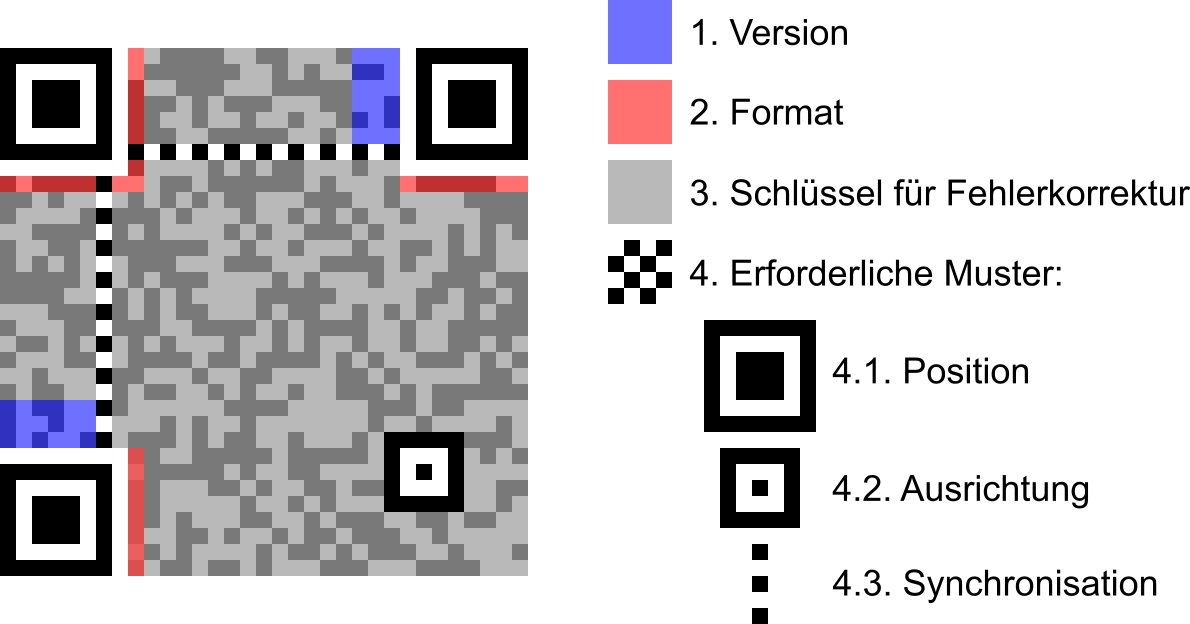
\includegraphics[scale=0.3]{images/QR_Code_Struktur_Beispiel.png}
\label{fig:struktur-qrcode}\caption{\QRCode Strukturbeispiel (siehe Quelle \cite{qrcoderef})}
\end{figure}


Des weiteren ist klar zu erkennen, dass der Code in drei von vier Ecken das Muster 4.1 vorweist. Diese dienen zur Bestimmung der Orientierung. Zusätzlich wird das Muster 4.2 (\emph{Finder Pattern}) verwendet um die Ausrichtung noch prezieser zu bestimmen. Bei größeren \QRCodes werden weitere Ausrichtungsmuster (Muster 4.2) eingefügt. Zwischen den \emph{Finder Patterns} befindet sich ein Streifen mit abwechselnd \glqq schwarz - weißen\grqq\  Punkten (\emph{Modulen}). Das sind die so genannten Synchronisations Muster oder auch \emph{Timming Patterns}.

Die Größe der \QRCodes ist beschränkt durch die Anzahl der \emph{Module}. Die Anzahl der \emph{Module} liegt zwischen $21 \times 21$ und $177 \times 177$. Beispielsweise sei der Code in Abbildung \ref{fig:struktur-qrcode} einer der Größe $21 \times 21$. Dann hätte ein \emph{Finder Pattern} die länge von $7$ \emph{Modules}. Die Anzahl ergibt sich aus der einzigartigen $1:1:3:1:1$ Struktur eines \emph{Finder Patterns}. Diese Fakten werden später ausschlagegebend sein bei der Rasterisierung des \QRCodes.

\section{Die verwendette Bibliothek OpenCV}
\OpenCV\footnote{WWW-Seite von dem Projekt \OpenCV: \url{http://opencv.org/}} ist eine Bibliothek mit Algorithmen spezialisiert auf \glqq Computer Vision\grqq . Sie wurde für die Programmiersprachen C/C++ geschrieben und steht unter BSD Lizenz. Es gibt mehrere Versionen der Bibliothek, die aktuellste ist die 3.2. Unser Programm setzt  die mindestanforderung auf Version 2.4. Außer \OpenCV wurde keine weitere Bibliothek verwendet. 




\cleardoublepage
\chapter{Bildvorverarbeitung}
Die Bildvorverarbeitung stellt ein essenziellen Schritt zur Lokalisierung der \QRCodes dar. Das Eingabebild wird in dieser Phase zuerst in ein Graustufenbild umgewandelt und danach binarisiert. Der Einfachheit halber werden zu große Bilder zuerst noch auf unter 1500 in der größten Dimension verkleinert. \OpenCV bietet die Möglichkeit Bilder direkt als Graustufenbild einzulesen, welches für Schwellenwertoperationen genutzt wird.
Die Klasse \texttt{ImageBinarization} ist für die darauf folgende Binarisierung zuständig. 
\inputCPP[label={lst:binarize}][][Ablauf der Binarisierung.]{code/binarize-run.cpp}

In Zeile 4 wird die Methode \texttt{computeSmoothing} aufgerufen, die eine Gaußglättung auf dem Bild durchführt, um den Einfluss von Rauschen zu mindern. Um mit verschiedenen Belichtungsszenarien umgehen zu können, sind drei Methoden zur Schwellwertberechnung implementiert:
\begin{itemize}
	\item Globales Schwellwertverfahren
	\item Mittelwert-Schwellwertverfahren
	\item Gaußsches-Schwellwertverfahren
\end{itemize}
\inputCPP[label={lst:globalthreshold}][][Binarisierung anhand des globalen Schwellwertverfahrens.]{code/global-binarize.cpp}
Im ersten Durchlauf wird das globale Schwellwertverfahren angewandt. Bei der Berechnung wird auf die \texttt{threshold} Methode, wie sie im Listing \ref{lst:globalthreshold} steht, zurückgegriffen. Diese verwendet den \emph{Otsu} Algorithmus\footnote{Mehr Information zu dem Algorithmus auf der zugehörigen \OpenCV Seite:\url{http://docs.opencv.org/2.4/modules/imgproc/doc/miscellaneous_transformations.html\#threshold}}, um einen globalen Schwellwert zu berechnen und dann das Bild zu binarisieren.

Sollte diese Methode nicht mindestens drei \fps lokalisieren, wird das nächste Verfahren ausgeführt.

\inputCPP[label={lst:localthreshold}][][Binarisierung anhand eines lokalen Schwellwertverfahrens.]{code/local-binarize.cpp}

Bei den lokalen Schwellwertverfahren wird die Methode \texttt{adaptiveThreshold} verwendet, welche in Listing \ref{lst:localthreshold} veranschaulicht wird. Im Gegensatz zum globalen Schwellwertverfahren, wird hier für jeden Pixel anhand der Nachbarschaft ein eigener Schwellwert errechnet. Als empirisch gut geeignet hat sich eine Nachbarschaft von $11 \times 11$ herausgestellt.

Die Berechnung des Schwellwerts für die Nachbarschaft erfolgt auf zwei unterschiedliche Verfahren:
\begin{description}
	\item[\texttt{ADAPTIVE\_THRESH\_MEAN\_C}:] Der Mittelwert der Nachbarschaft.
	\item[\texttt{ADAPTIVE\_THRESH\_GAUSSIAN\_C}:] Ein Gauß gewichteter Mittelwert der Nachbarschaft.
\end{description}

Der Parameter \texttt{C} wird vom Mittelwert subtrahiert. In der Implementierung wird \texttt{C} konstant $0$ gewählt.

\begin{figure}[h]
\center

\includegraphics[scale=0.12]{images/qrcode-adler-wand_1___BINARIZED___.jpg}
\hspace{5px}

\includegraphics[scale=0.12]{images/qrcode-adler-wand_2___BINARIZED___.jpg}
\caption{Das Resultat der Binarisierung mit den jeweiligen Verfahren. Links global und Rechts lokal.}
\end{figure}
\cleardoublepage
\chapter{Patternidentifikation}
Der nächste Schritt auf dem Weg zur Lokalisierung der \QRCodes ist das Identifizieren der \fps. Dafür wird die durch \OpenCV bereitgestellte \texttt{findContours} Methode verwendet. Sie basiert auf dem Algorithmus von Suzuki und wird eingesetzt, um die Konturen aus dem Binärbild zu bestimmen.
\inputCPP[label={lst:findcontours}][][Aufruf der \texttt{findContours} Methode um die Konturen zu bestimmen.]{code/findContours.cpp}
Listing \ref{lst:findcontours} zeigt den Aufruf um alle Konturen des übergebenen Bildes zu erhalten.

\section{Vorgehensweise des Algorithmus von Suzuki} \label{suzuki}
Das Binärbild wird als durch iterriert. Für jeden Pixel $p_{i,j}$ werden folgende Bedingungen überprüft:
\begin{description}
	\item[outer border] Falls der Farbton des Vorgängers sich vom aktuell betrachteten Pixel unterscheidet. Beispielsweise für den Pixel $p_{i,j} = 1$ und $p_{i,j-1} = 0$ wäre $p_{i,j}$ ein Startpunkt einer \emph{outer border}. 
	\item[hole border] Falls der Farbton der Vorgänger sich in einem bestimmten Abstand gleich war, aber im aktuellen Pixel $p_{i,j}$ unterscheidet. Sei $x > 1$ ein beliebiger Abstand und es gelte $p_{i,j-x} =\ldots = p_{i,j-1}= 1$ und $p_{i,j} = 0$, dann ist $p_{i,j}$ ein Startpunkt einer \emph{hole border}.
\end{description}
Sind beide Bedingungen erfüllt, ist der Pixel $p_{i,j}$ ein Anfangspunkt einer neuen Kontur. Diese Kontur muss eindeutig identifizierbar sein daher wird sie mit einer \emph{KonturID} versehen. Der große Vorteil dieses Algorithmus ist die abgespeicherte Hierarchie der Konturen. Um dies zu gewährleisten, muss die \emph{parent}-Kontur für die neue Kontur gesetzt werden. Während des Scannens des Bildes wird immer die äußere Kontur zwischengespeichert, diese ist entweder die \emph{parent}-Kontur oder die Kontur die, die neue Kontur und die \emph{parent}-Kontur teilt. Wenn alle Werte gesetzt sind, wird die Kontur durch sukzessives Hinzunehmen von Pixeln entlang der Kante erzeugt. Das heißt es wird eine Kantenverfolgung durchgeführt. Nach jeder Kontur Erzeugung springt der Algorithmus zurück zum Raster Scan. Der Algorithmus terminiert bei Erreichen der rechten unteren Ecke.

Das Orginal Paper \cite{journals/cvgip/SuzukiA85} beschreibt ausfürlich das Vorgehen anhand Beispielen und Pseudocode.

\section{Filtern der Konturen}
Nachdem die Konturen bestimmt wurden, müssen die Konturen gefiltert werden da abhängig vom Bild können eine variable Anzahl an Konturen
erkannt werden. Beispielsweise werden bei der Ausführung der adaptiven Schwellwertoperation viele kleine Konturen erkannt. In folgenden Fällen werden Konturen ignoriert, da sie keine Aussagekraft besitzen.
\begin{enumerate}
	\item Die Kontur ist zu klein oder zu groß.
	\item Die Kontur besitzt kein \emph{parent}-Kontur.
	\item Konturen die Nachbarkonturen besitzen.
	\item Konturen die eine \emph{child}-Kontur besitzen.
\end{enumerate}
Für die äußeren Konturen also die \emph{parent}-Konturen müssen die Bedingungen 1.-3. natürlich auch gelten. Zusätzlich muss für die äußerste Kontur eine Trapezoide Form gelten. Um die letzte Bedingung zu überprüfen wird dazu die Form der Kontur mit \texttt{approxPolyDP} Methode approximiert und wenn diese aus genau vier Punkten besteht, wird es als Trapezoid anerkannt.

\section{Kanten approximieren}
Nachdem mehrere Kandidaten von \fps gefunden wurden, wird als nächstes die äußerste Kontur dieser Kandidaten verwendet um deren Kanten zu approximieren. Zuvor haben wir mit \OpenCV und Suzukis Algorithmus \ref{suzuki} alle Konturen mit \texttt{CV\_CHAIN\_APPROX\_NONE} im Bild lokalisiert, weswegen jede Kontur jetzt eine zusammenhängende Kette von Punkten darstellt. Für jeden Kandidat soll mit Hilfe dieser Punktmenge die Vier äußeren Kanten des \fps approximiert werden. Dazu teilen wir die Kontur in Vier Segmente auf und benutzen diese im späteren Verlauf um die Kanten zu approximieren.

\begin{figure}[h]
\centering
\begin{subfigure}[t]{0.48\textwidth}
\centering
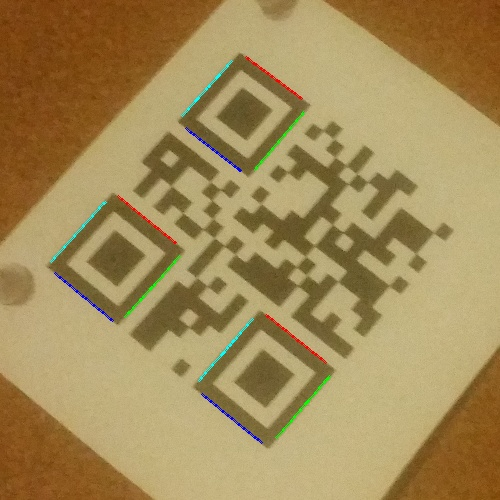
\includegraphics[scale=0.25]{images/qrcode-adler-wand_4___SEGMENTS___.jpg}
\caption{Segmentierung}
\end{subfigure}%
\begin{subfigure}[t]{0.48\textwidth}
\centering
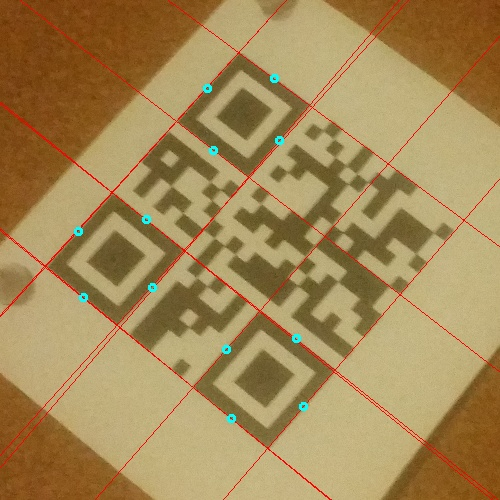
\includegraphics[scale=0.25]{images/qrcode-adler-wand_5___LINES___.jpg}
\caption{Geraden Approximation}
\label{fig:lines}
\end{subfigure}
\caption{Aufteilen der einzelnen \fp Konturen in Segmente und Approximation der Kanten durch Geraden.}
\end{figure}

Um die Schnittpunkte zu finden, an welchen die Kontur geteilt werden muss, werden die zuvor berechneten Vier Punkte, welche bereits genutzt wurden um festzustellen ob es sich bei der Kontur um ein Trapezoid handelt, verwendet. Diese liegen jedoch im Regelfall nicht exakt auf den Ecken der \fps und zusätzlich kann es durch schlechte Bildqualität zu abgerundeten oder leicht verschobenen Ecken im Originalbild kommen. Deswegen wird nachdem die Kontur zerteilt wurde, jeweils 10\% aller Punkte am Anfang und Ende jedes Segments verworfen, sodass ein Segment nur noch 80\% aller Punkte einer Kante beinhaltet. Diese Segmente werden dann genutzt um mit der \texttt{fitLine}-Methode die Kanten zu approximieren.

Die \texttt{fitLine}-Methode beruht auf dem Prinzip von \emph{M-Estimators} und verwendet als Minimierungsfunktion den in \OpenCV durch \texttt{CV\_DIST\_FAIR} definierten Ausdruck. Eine wichtige Eigenschaft dieser Methode ist, dass sie Geraden als einen Stützvektor und einen Richtungsvektor darstellt und der Stützvektor die Eigenschaft hat, sich innerhalb der konvexen Hülle aller Punkte zu befinden, welche zur Approximation verwendet wurden.
\\\\
Am Ende der Identifikation aller möglichen \fps erhält man somit folgende Informationen:
\begin{itemize}
	\item Mindestens drei \fp Kandidaten
	\item Eine Kontur pro \fp
	\item Vier Segmente pro \fp
	\item Vier Kantengeraden pro \fp
\end{itemize}
\cleardoublepage
\chapter{Extrahierung}

Der nächste Schritt auf dem Weg zum finden eines gültigen \QRCodes besteht darin, alle Möglichen Dreier-Kombinationen von \fps zu prüfen und festzustellen, ob diese zur Extrahierung eines gültigen \QRCodes führen. Für jede Kombination wird versucht, die vier Eckpunkte des \QRCodes zu berechnen, um aus diesem eine Matrix für eine perspektivische Transformation in eine 2D-Ebene zu berechnen. Dies führt zu $\binom{k}{3}$ möglichen Kombinationen von \fps, wobei $k$ die Anzahl aller gefundenen \fps ist.

\section{Pattern Positionierung}
Hat man drei \fps ausgewählt, muss für die korrekte Extrahierung festgestellt werden, welche Position im \QRCode jedes \fp einnimmt.

Zuerst werden dazu die \fps durch Verwendung der Gaußschen Trapezformel im Uhrzeigersinn angeordnet.
\begin{theorem}[Gaußsche Trapezformel]
Berechnet den Flächeninhalt eines einfachen Polygons.
\begin{align}
A=\frac{1}{2} \sum_{0}^{n-1} (y_i + y_{i+1\ mod\ n})(x_i - x_{i+1\ mod\ n})
\end{align}
\end{theorem}
Dabei ist $n$ die Anzahl der Punkte in einem Polygon und $x_i$ und $y_i$ die Punktkoordinaten des $i$-ten Punkts. Abhängig vom Drehsinn der Punkte im Bezug auf das Koordinatensystem ist der Flächeninhalt entweder positiv oder negativ. In einem kartesischen Koordinatensystem entspricht ein positiver Flächeninhalt einem Drehsinn im Uhrzeigersinn und ein negativer gegen den Uhrzeigersinn.

Angewendet wird die Formel auf das Polygon, welches aus dem jeweils ersten Punkt der Kontur jedes \fps besteht. Ist der Flächeninhalt negativ wird die Reihenfolge geändert, indem das erste und zweite \fp miteinander vertauscht werden.
\subsubsection{Ähnlichkeitsmaß für Geraden}
Sind die \fps in korrekter Reihenfolge, wird als nächstes das \olfp bestimmt. Zurzeit sind durch die drei \fps insgesamt 12 approximierte Geraden bekannt. Betrachtet man den Aufbau eines \QRCodes, ist ersichtlich das jeweils 4 Geradenpaare die selbe Kante beschreiben. Es gibt insgesamt also nur 8 unterschiedliche Kanten und nur das \olfp teilt sich jede Kante mit einem anderen \fp. Die anderen beiden \fps teilen sich je nur 2 Kanten mit dem \olfp. Stellt man also fest welche der 12 Geraden die gleichen Kanten im \QRCode approximieren, ergibt sich welches \fp das \olfp ist.

Für das effiziente Zuordnen von Geraden wird ausgenutzt, dass die Stützvektoren der Kantengeraden stets im Mittelpunkt der Segmente liegen durch welche sie approximiert wurden. Die Ähnlichkeit von zwei Geraden wird dann definiert über die Summe der Entfernung des Stützvektors der ersten Gerade zur zweiten Gerade und umgekehrt.

\inputCPP[label={lst:similarity}][][Ähnlichkeitsmaß für zwei Geraden]{code/similarity.cpp}

\begin{wrapfigure}{R}{0.4\textwidth}
  \vspace{-20pt}
  \begin{center}
    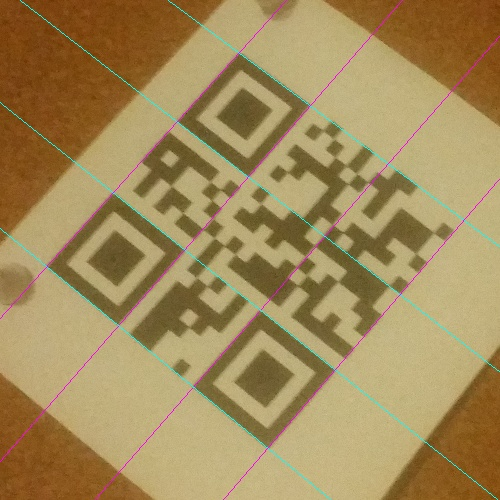
\includegraphics[scale=0.25]{images/qrcode-adler-wand_6___SPLIT___0_.jpg}
  \end{center}
  \vspace{-10pt}
  \caption{Zuordnung der Geraden zu horizontalen oder vertikalen Kanten.}
  \vspace{-10pt}
\end{wrapfigure}

Ein kleinerer Wert bedeutet bei dieser Definition das sich zwei Geraden besonders ähnlich sind. In Abbildung \ref{fig:lines} ist dabei gut zu erkennen, dass wenn es sich um einen \QRCode handelt, welcher mit ausreichend guter Qualität für eine korrekte Kantenapproximation abgebildet ist, sich dieses Maß ausreichend gut eignet um festzustellen, welche Geraden die selbe Kante approximieren. Für das \olfp gilt dann, dass es das \fp mit den vier kleinsten Ähnlichkeitsmaßen ist.

Da zuvor die \fps im Uhrzeigersinn angeordnet wurden, können wir durch Rotation im Uhrzeigersinn nicht nur das \olfp an die erste Stelle des Pattern Arrays bringen, sondern wissen auch direkt das sich an der zweiten Stelle das \orfp und an der dritten Stelle das \ulfp befindet. Mit Ausnahme für Spiegel verkehrte \QRCodes kann zuverlässig die korrekte Position aller \fps im \QRCode bestimmt werden.

\begin{figure}[h]
\center
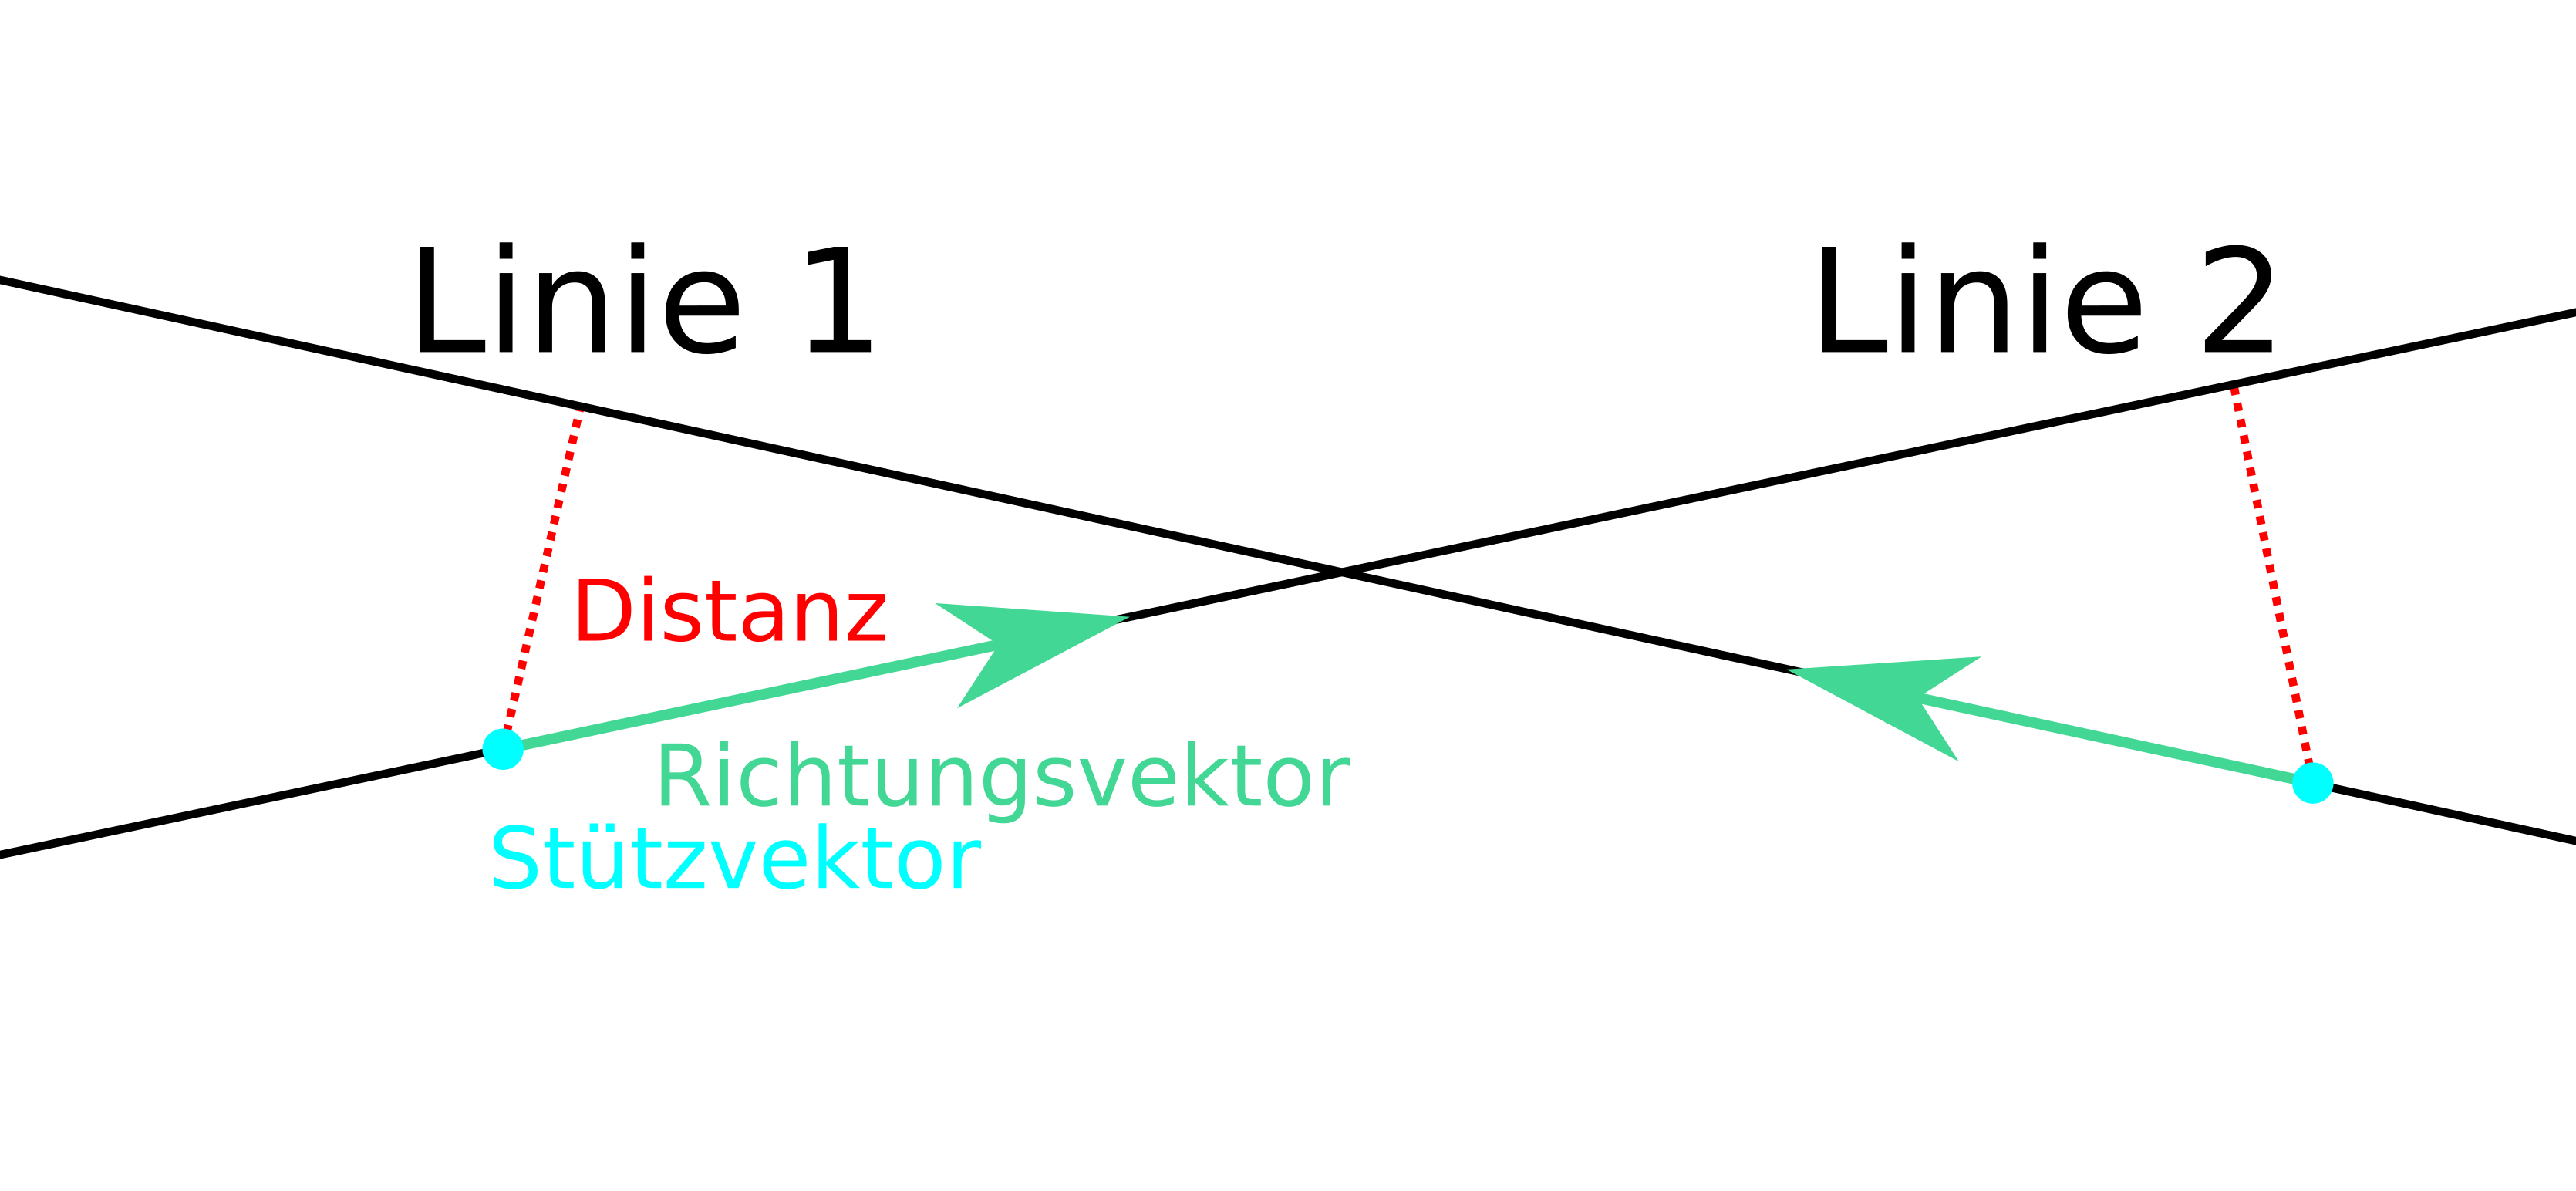
\includegraphics[scale=1]{images/similarity_measure.png}
\caption{Links: Ähnlichkeitsmaß von zwei Geraden.}
\end{figure}

\section{Kanten Zuordnung}
Um die Eckpunkte des \QRCodes durch Schnittpunktbildung der äußeren Kanten zu berechnen, muss als nächstes festgestellt werden, welche Geraden die Außenkanten des \QRCodes beschreiben.

\subsubsection{Vertikale und Horizontale Geraden}
Da bereits berechnet wurde, welche der Geraden die selbe Kante approximieren, kann diese Information benutzt werden um eine qualitativ bessere Approximation für alle Kanten des \olfp zu berechnen. Dazu werden die zugrunde liegenden Segmente von den gepaarten Geraden genommen und auf der Vereinigung dieser Segmente wird erneut der Approximationsprozess ausgeführt. Indem dabei festgestellt wird ob mit einer Geraden aus dem \orfp oder dem \ulfp vereinigt wird, ergibt sich ob die neue Gerade im \QRCode Koordinatensystem eine horizontale oder vertikale Kante beschreibt. Die nicht verwendeten Kanten am Ende des Prozesses sind danach ebenfalls trivial zuzuordnen. Falls an dieser Stelle nicht genau je zwei Geradenpaare von \olfp und \orfp, sowie zwei Geradenpaare von \olfp und \orfp vereinigt wurden, ist die Kombination von \fps kein \QRCode und es kann abgebrochen werden.

War die Vereinigung erfolgreich gibt es genau vier horizontal und vier vertikal zugeordnete Geraden.

\subsubsection{Sortieren der Geraden}
Danach werden die horizontalen Geraden entlang einer beliebigen vertikalen Gerade sortiert, welche von nun an als Sortier-Achse bezeichnet wird. 

Wie in Abbildung \ref{fig:sort} gezeigt, werden dazu alle Schnittpunkte zwischen der Sortier-Achse und den horizontalen Geraden berechnet. Dann wird eine Koordinatensystem Transformation ausgeführt, sodass die Sortier-Achse zur neuen X-Achse des Koordinatensystems wird. Somit können die horizontalen Geraden nach der Größe der X-Werte der Schnittpunkte mit der Sortier-Achse sortiert werden. Zuletzt wird festgestellt ob das erste Element der so sortierten Liste von horizontalen Geraden mit einer Gerade des \olfp übereinstimmt. Falls nicht wird die Liste umgedreht.

Für die vertikalen Geraden kann dies analog durchgeführt werden. Diese Methode wurde gewählt, um sicherzustellen das unabhängig von perspektivischen Verzerrungen die Sortierreihenfolge stabil bleibt.

\begin{figure}[h]
\centering
\begin{subfigure}[t]{0.48\textwidth}
\centering
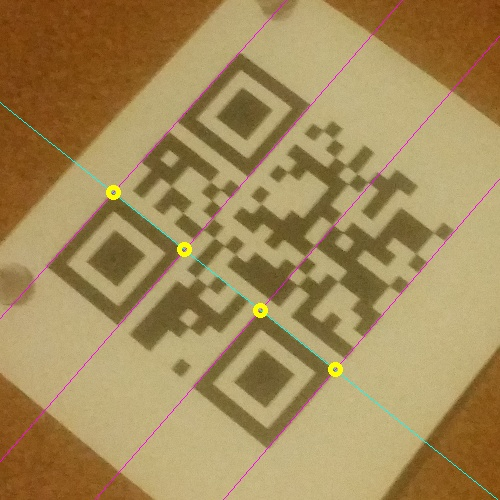
\includegraphics[scale=0.25]{images/qrcode-adler-wand_7___SORT___0_.jpg}
\caption{Schnittpunkte entlang der Sortier-Achse}\label{fig:sort}
\end{subfigure}%
\begin{subfigure}[t]{0.48\textwidth}
\centering
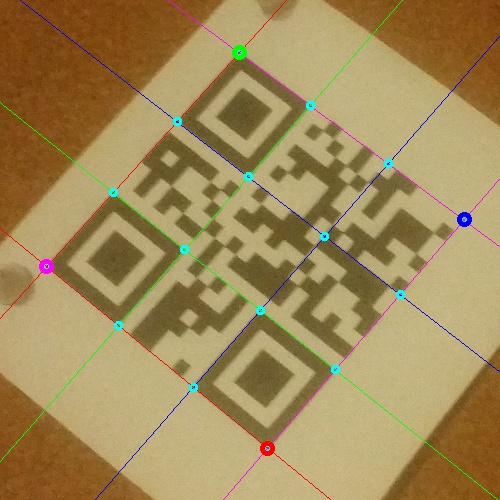
\includegraphics[scale=0.25]{images/qrcode-adler-wand_9___INTERSECTIONS___0_.jpg}
\caption{Schnittpunkte aller horizontalen und vertikalen Geraden}
\end{subfigure}
\caption{Sortieren aller Geraden entlang einer Achse und Berechnung der Eckpunkte.}
\end{figure}

Das Ergebnis sind zwei Listen von Geraden die im \QRCode Koordinatensystem von oben links nach unten rechts sortiert sind. Dementsprechend können nun trivial die Schnittpunkte der ersten und letzten Geraden berechnet werden, wodurch die Eckpunkte des \QRCodes bestimmt werden. Mit diesen vier Punkten und der \OpenCV Funktion  \texttt{getPerspectiveTransform} sowie \texttt{warpPerspective} wird dann eine perspektivische Transformationsmatrix errechnet und der \QRCode extrahiert.
\cleardoublepage
\chapter{Normalisierung}
\section{Rasterisierung}

\begin{wrapfigure}{R}{0.4\textwidth}
  \vspace{-20pt}
  \begin{center}
    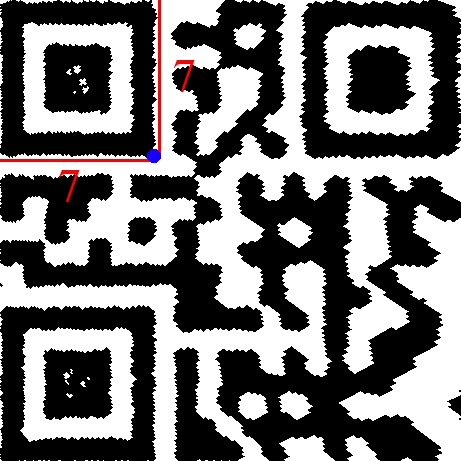
\includegraphics[scale=0.25]{images/Gitter_step.png}
  \end{center}
  \vspace{-10pt}
  \label{fig:raster-qrcode}\caption{Rasterlänge berechnen}
  \vspace{-10pt}
\end{wrapfigure}

Nach der perspektivischen Transformation, liegt das Bild in einem $n\times n$ großem binärisiertem Zustand vor. Nun muss der \QRCode rasterisiert werden. 
Man betrachte dazu die untere rechte Ecke des oberen linken Finder Pattern. Es ist bekannt, dass ein Finder Pattern die Dimension $7 \times 7$ hat,
sodass man die $x$ bzw. $y$-Koordinate der genannten Ecke durch $7$ dividiert.

Dies liefert die Zellenlänge $z$ des Rasters,
woraus sich die Anzahl der Module $m$ via Division von $n$ mit $z$ berechnen lässt. Im Normalfall gilt jedoch $m \notin \mathbb{Z}$.
Es ist jedoch bekannt, dass ein \QRCode nur 
\begin {equation*}
	17 + 4 \cdot version,
\end{equation*}
für $version \in \left\{1, ..., 40\right\} \subset \mathbb{N}$, Module besitzen kann.

\todo{Quelle angeben!}
%\footnote{Quelle: \url{http://www.qrcode.com/en/img/version/versionVarietyImage.png}
\begin{figure}[h]
\centering
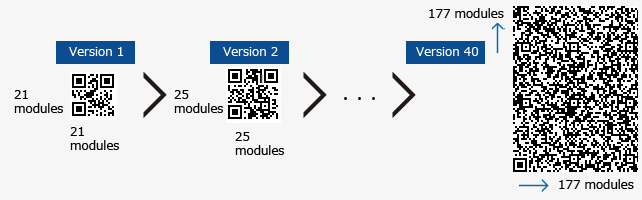
\includegraphics[scale=0.5]{images/QRVersion.png}
\label{fig:version-qrcode}\caption{Mögliche Modulgrößen von QR-Codes} 
\end{figure}
\\
Man runde die Anzahl der berechneten Module $m$ auf die nächstliegende Versionsnummer via
\begin{equation*}
	version = cvRound((m-17)/4);
\end{equation*}
Die zugehörige Anzahl der Module ist dann also gegeben durch
\begin{equation*}
	modules = 17+4 \cdot version;
\end{equation*} 
Die Zellenlänge des Rasters berechnet sich letztendlich aus Divison von $n$ mit $modules$. Diese Zellenlänge wird für den folgenden Schritt der Normalisierung benötigt.

\section{Normalisierung}
Die Normalisierung wird mithilfe des Rasters durchgeführt, indem majority votes pro Zelle den Pixelwert des normalisierten \QRCodes festlegen.
Das Ergebnis ist also ein $modules \times modules$ großer normalisierter \QRCode.
\begin{figure}[h]
\centering
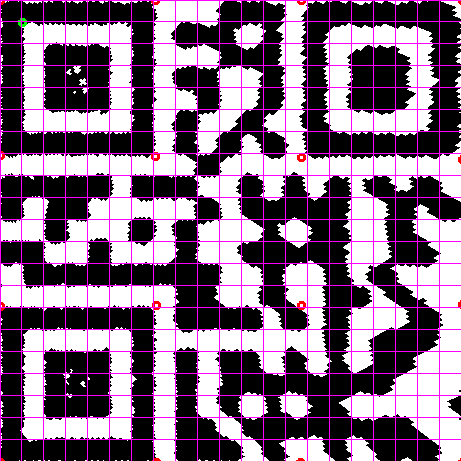
\includegraphics[scale=0.25]{images/gitter.png}
\label{fig:version-qrcode}\caption{Normalisierung des \QRCodes}
\end{figure}

\section{Verifikation}
Um fälschlicherweise erkannte \QRCodes zu vermeiden, wird im Anschluss noch eine Verifikation durchgeführt. Dies geschieht, indem die Pixel des normalisierten Bildes, an denen die Finder Patterns und Timing Patterns liegen, mit den Finder bzw. Timing Patterns eines Standard \QRCodes verglichen werden.
\begin{figure}[h]
\centering

\includegraphics[scale=0.5]{images/verifikation.png}
\label{fig:version-qrcode}\caption{Finder und Timing Patterns eines Standard \QRCode}
\end{figure}
\\
Ist die Übereinstimmung des normalisierten Bildes mit einem Standard \QRCode geringer als $85\%$, so wiederhole, falls möglich, die Normalisierung und die Verifikation mit einer Versionsnummer von $\pm 1$, um falsche Rundungen bei der Rasterisierung vorzubeugen.
\\
Sind alle Übereinstimmungen unter $65\%$, so wird der \QRCode verworfen, andernfalls wird der \QRCode mit der höchsten Übereinstimmung gewählt und schlussendlich ausgegeben.

\cleardoublepage
\chapter{Evaluierung}

Um den implementierten Algorithmus zu testen, werden sowohl reale als auch synthetische Datenbanken verwendet. Die generierte synthetische Datenbank stellt eine Vielzahl von verschiedenen Testbildern bereit. Ein großer Vorteil daran ist, dass die Parameter der generierten Testbilder manuell eingestellt werden können, sodass eine einfache Analyse, unter welchen Umständen die implementierte QR Detektion scheitert, möglich ist.

\section{Ablauf der synthetischen Generierung}

\texttt{Input}: Menge von groundtruth \QRCodes \\
\texttt{Output}: Datenbank von synthetischen Bildern

\begin{enumerate}
	\item Randerstellung
	\item Skalierung
	\item Rotation
	\item Perspektivische Transformation
	\item Einbettung in Hintergründe
	\item Gaußglättung
	\item Rauschen
\end{enumerate}

%Hier Bilder für Generierung hinzufügen?

Pro Schritt kann festgelegt werden, wie viele Dateien generiert werden sollen.
Einzelne Schrittweiten und Maximalwerte können angegeben werden, beispielsweise:
\begin{enumerate}
	\item Rotation: Diskretisierung in $45$ Schritten
	\item Gaußglättung: Startwert von $n=3$, Schrittweite von $6$, Maximalwert von $n=27$
	\item ...
\end{enumerate}

\textbf{Verbesserungen der synthetischen Datenbank}\\
Die synthetische Datenbank kann um viele Aspekte erweitert werden. So können unterschiedliche Belichtungen simuliert werden, oder Stellen der \QRCodes „verdeckt“ werden oder auch Wölbungen generiert werden. Auch könnte man mehr als ein \QRCode in ein Bild einbetten.
Ebenfalls wäre es möglich Testbilder zu generieren, welche Aussagen über die false-positive Rate der QR Detektion treffen. Das heißt Bilder generieren, welche keine \QRCodes aber Formen, die den Finder Pattern ähnlich sind, enthalten.

\section{Evaluation}

\textbf{Evaluation der synthetischen Datenbank} \\
\begin{tabular}{l c c c c}
 		& Anzahl & Erkannt & Qualität & Parameter \\
		Skalierung & $60$ & $60$ & $98\%$ & $6$,IL, IN \\
		Rotation  & $420$ & $420$ & $97.35\%$ & $0<r<360$, $45$\\
		Perspektive & $1000$ & $935$ & $95.6\%$ & $0 \leq x,y<0.3$, $0.1$\\
		Einbettung & $300$ & $268$ &  $96.82$ & $60\%$\\
		Glättung & $200$ & $131$ & $94.4\%$ &  $5\leq n \leq 23$, $6$\\
		Rauschen & $200$ & $116$ & $95.24\%$ & $15 \leq \sigma \leq 45$, $15$\\
\end{tabular}
\\ \\
%Bearbeite diese Legende, so unschön
Skalierung: Skalierungsfaktor $6$, IL $=$ lineare Interpolation, IN $=$ nearest neighbour Interpolation\\
Perspektive: Position der oberen linken Ecke in Prozent bzgl. Dimension des Bildes \\
Einbettung: Größe des \QRCodes innerhalb des Hintergrundes \\

\textbf{Evaluation von realen Datenbanken} \\


%Diese Evaluation nochmals durchführen und werte übertragen! Laufzeit bzgl welchen Systems?
\begin{tabular}{l c c c c}
 		& Anzahl & Erkannt & Erkennungsrate & Laufzeit \\
		dataset1 & $410$ & $227$ & $55.3\%$ & $100$s \\
		dataset2 & $400$ & $300$ & $75\%$ & $20$s \\
\end{tabular}
\\ \\
Die Erkennungsrate bei dem \emph{dataset1}\footnote{Quelle: \url{http://www.fit.vutbr.cz/research/groups/graph/pclines/pub_page.php?id=2012-JRTIP-MatrixCode} [dataset1.zip] [dataset2.zip]} ist relativ niedrig, denn der Algorithmus scheiterte an der zu kleinen  \emph{Quietzone}.
Die Schneidung von Text mit dem \QRCode führt zu einer Problematik bei der Konturdetektion. Ebenfalls scheiterte die Detektion an zu starken unebenen Belichtungen. Beispielsweise ein Schatten, der quer durch den \QRCode verläuft.
Bei dem \emph{dataset2} scheiterte der Algorithmus ebenfalls an der zu kleinen \emph{Quietzone}. \\ \\


\textbf{Probleme der implementierten QR Detektion} \\
Der implementierte Algorithmus hat Probleme unter den folgenden Bedingungen:
\begin{enumerate}
\item Stark unebene Belichtungen: Obwohl adaptive Schwellenwerte verwendet werden, wird das Bild nicht optimal binärisiert. Dies liegt höchstwahrscheinlich daran, dass die Parameter des adaptiven Schwellenwertes nicht optimal eingestellt sind. 

\item Zu kleine Quietzone: Falls die Quietzone zu klein ist, kann es vorkommen, dass die Konturen der Finder Patterns nicht richtig erkannt werden. Die gefundene Kontur verläuft dann oftmals durch die Umgebung des FinderPatterns.
\end{enumerate}
%Hier vielleicht Problembilder einfügen?





\textbf{Ausblick:} Durch das verändern des Parameters \texttt{C} in der \texttt{adaptiveThreshold} Methode kann eine ausgeglichenere Binarisierung erzielt werden. Allerdings können aus leicht Informationen verloren gehen!



\printbibliography

\end{document}
